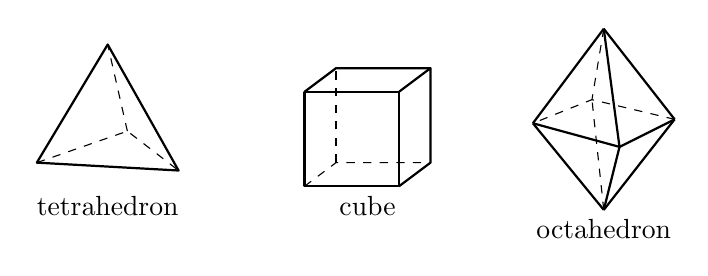
\begin{tikzpicture}[scale=1, line join=round]
  % tetrahedron
  \begin{scope}[shift={(0,0)}]
    \coordinate (T1) at (-0.9,-0.5); \coordinate (T2) at (0.9,-0.6);
    \coordinate (T3) at (0.25,-0.1); \coordinate (T4) at (0,1.0);
    \draw[thick] (T1) -- (T2) -- (T4) -- cycle;
    \draw[dashed] (T1) -- (T3) -- (T2); \draw[dashed] (T3) -- (T4);
    \node[below] at (0,-0.8) {tetrahedron};
  \end{scope}
  % cube
  \begin{scope}[shift={(3.2,-0.2)}]
    \coordinate (C1) at (-0.7,-0.6); \coordinate (C2) at (0.5,-0.6);
    \coordinate (C3) at (0.5,0.6); \coordinate (C4) at (-0.7,0.6);
    \coordinate (D1) at (-0.3,-0.3); \coordinate (D2) at (0.9,-0.3);
    \coordinate (D3) at (0.9,0.9); \coordinate (D4) at (-0.3,0.9);
    \draw[thick] (C1) -- (C2) -- (C3) -- (C4) -- cycle;
    \draw[thick] (C2) -- (D2) -- (D3) -- (C3); \draw[thick] (D3) -- (D4) -- (C4);
    \draw[dashed] (C1) -- (D1) -- (D2); \draw[dashed] (D1) -- (D4);
    \node[below] at (0.1,-0.6) {cube};
  \end{scope}
  % octahedron
  \begin{scope}[shift={(6.3,0)}]
    \coordinate (Ot) at (0,1.2); \coordinate (Ob) at (0,-1.1);
    \coordinate (O1) at (-0.9,0); \coordinate (O2) at (0.2,-0.3);
    \coordinate (O3) at (0.9,0.05); \coordinate (O4) at (-0.15,0.3);
    \draw[thick] (O1) -- (O2) -- (O3);
    \draw[dashed] (O3) -- (O4) -- (O1);
    \foreach \v in {O1,O2,O3} { \draw[thick] (Ot) -- (\v); \draw[thick] (Ob) -- (\v); }
    \draw[dashed] (Ot) -- (O4); \draw[dashed] (Ob) -- (O4);
    \node[below] at (0,-1.1) {octahedron};
  \end{scope}
\end{tikzpicture}
